\documentclass[xcolor=table]{beamer}

\usetheme[secheader,compress]{Madrid} %Primary theme

\usepackage{verbatim}
\usepackage{graphicx}

%% UTM Colors
\definecolor{UTMblue}{rgb}{0.043137, 0.137254, 0.254901}
\definecolor{UTMorange}{rgb}{1.0, 0.509803, 0}

\setbeamercolor{palette primary}{bg=UTMblue,fg=white}
\setbeamercolor{palette secondary}{bg=UTMblue,fg=white}
\setbeamercolor{palette tertiary}{bg=UTMblue,fg=white}
\setbeamercolor{palette quaternary}{bg=UTMblue,fg=white}
\setbeamercolor{structure}{fg=UTMblue} % itemize, enumerate, etc
\setbeamercolor{section in toc}{fg=UTMblue} % TOC sections
\setbeamercolor{title}{fg=UTMorange}

\setbeamercolor{subsection in head/foot}{bg=UTMorange,fg=white}

%%%%%%%%%%% BEGIN MACROS %%%%%%%%%%%%%%%%%%
% frameT: Frame with title
\newcommand{\frameT}[2]{\frame{\frametitle{#1} #2}}

% frameF: Fragile frame with title
\newcommand{\frameF}[2]{
  \begin{frame}[fragile]
    \frametitle{#1}
    #2
  \end{frame}
}

% frameTop: Frame aligned t the top
\newcommand{\frameTop}[2]{\frame[t]{\frametitle{#1} #2}}


\newcommand{\tab}{\hspace{1cm}}

\newcommand{\spaceor}{\hspace{5pt} \textbf{or} \hspace{5pt}}

\documentclass{beamer}
\usepackage{graphicx}
\usepackage{multicol}
\usepackage{multimedia}
\usepackage{hyperref}



%%%%%%%%%%% END MACROS %%%%%%%%%%%%%%%%%%%%



\begin{document}

\title{Bullet Blitz}

\author{Victor Gasior, Blade Johnson, Andrew Newbill, and Lucky Woods}
\institute{UT-Martin}
\date{\today}

%%%%%%%%%%% BEGIN TITLE %%%%%%%%%%%%%%%%%%
\frame{\titlepage}

 %\section{Outline}
%%%%%%%%%%%% END TITLE  %%%%%%%%%%%%%%%%%%

\section{Introduction}
\frameT{Motivation} {
  Motivations:
  \bigskip
  \begin{itemize}
  	\raggedright
    \item Classical FPS shooter game with inspiration from the game Quake as there have been a lower amount of arena shooters compared to the past couple decades.
      \bigskip
    \item The idea of the game is to have players be rodents like mice fighting each other with different kinds of weapons and jumping around the map.
  \end{itemize}

  \bigskip
  
  \emph{ 
} \emph{ }.
}


\frameT{Technology} {
  Technology used:
  \bigskip
  \begin{itemize}
    \item Unreal Engine 5: Used for the creation of the overall game.
    \begin{itemize}
      \item Ultimate Doom Builder: Used to create the maps used.
      \item Blender: Used to make the weapons used in the game along with helping import the maps.
    \end{itemize}
  \end{itemize}
  
  \bigskip
}


\frameT{Project Goals} {
  Goals:
  \begin{itemize}
      \item Networking testing to where players will be able to play together from different devices on the same server.
      \item Multiple weapons and Maps Available to the players.
      \item AI enemies available to substitute for players.
  \end{itemize}
  
  \bigskip
}

\section{Tools}

\frameT{Map Creation Pipeline} {
	\begin{center}
  		
\includegraphics[width=.8\linewidth]{figures/map_pipeline.png}
  	\end{center}
  	
  	\begin{multicols}{3}
        \begin{itemize}
        		\small
            \item The maps are made in Ultimate Doom Builder (UDB), they are exported into a .obj file.
            \item We import the .obj file into Blender, where we exported from Blender as an FBX file.
            \item Finally, the FBX file can be imported to UE as a model.
        \end{itemize}
    \end{multicols}
}

\frameT{Test Maps}{
	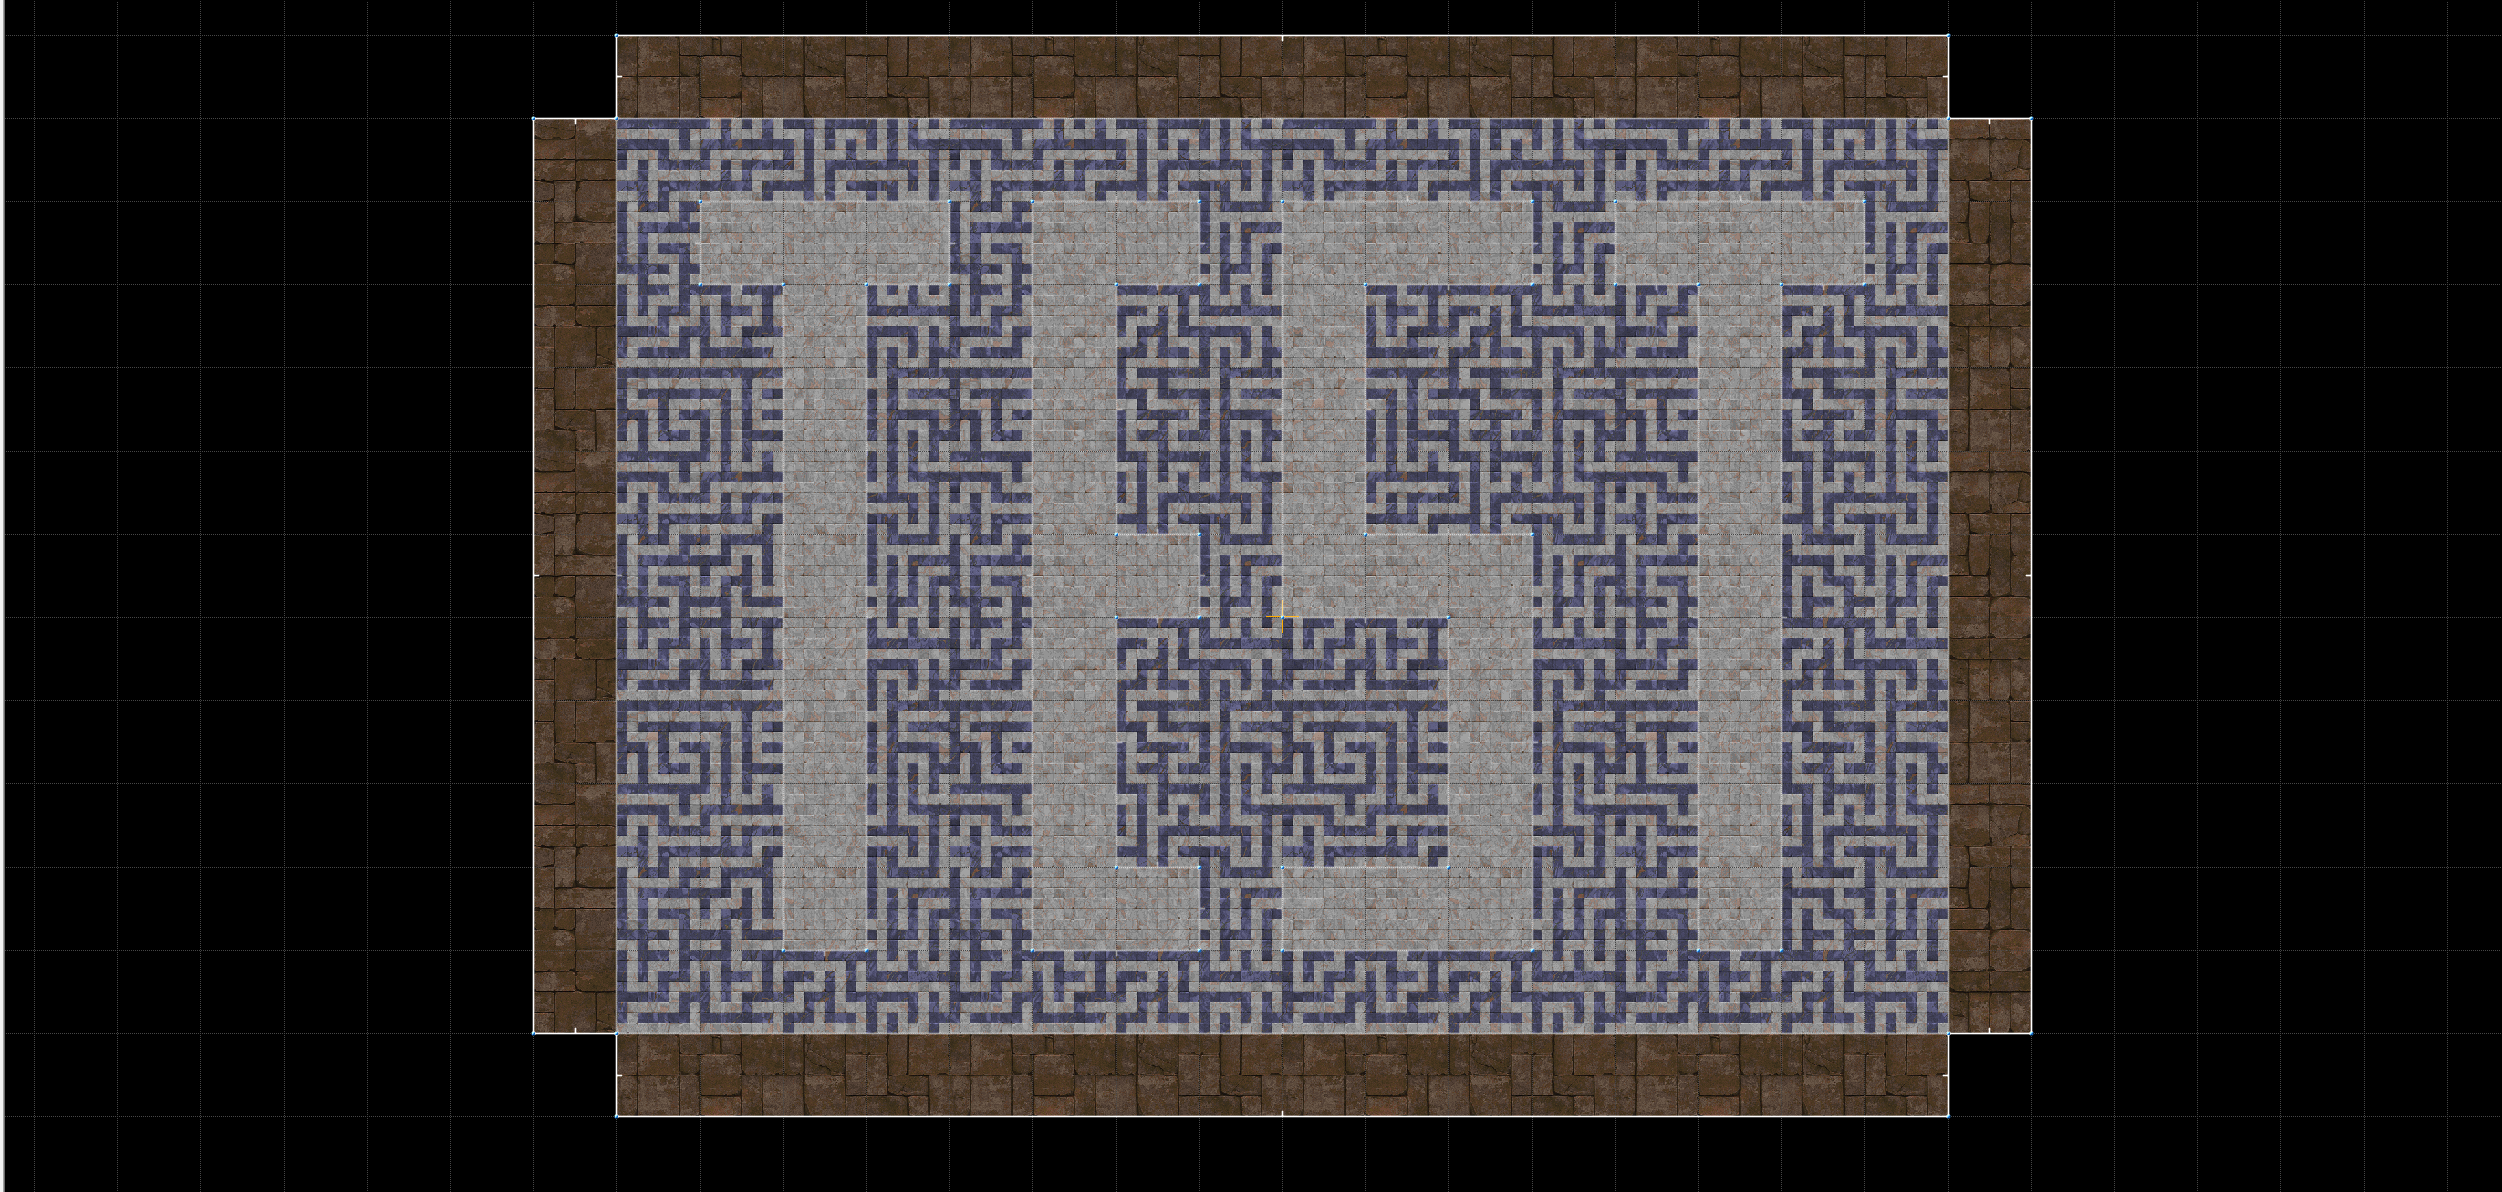
\includegraphics[height=.25\linewidth]{figures/test_map_doom.png}
	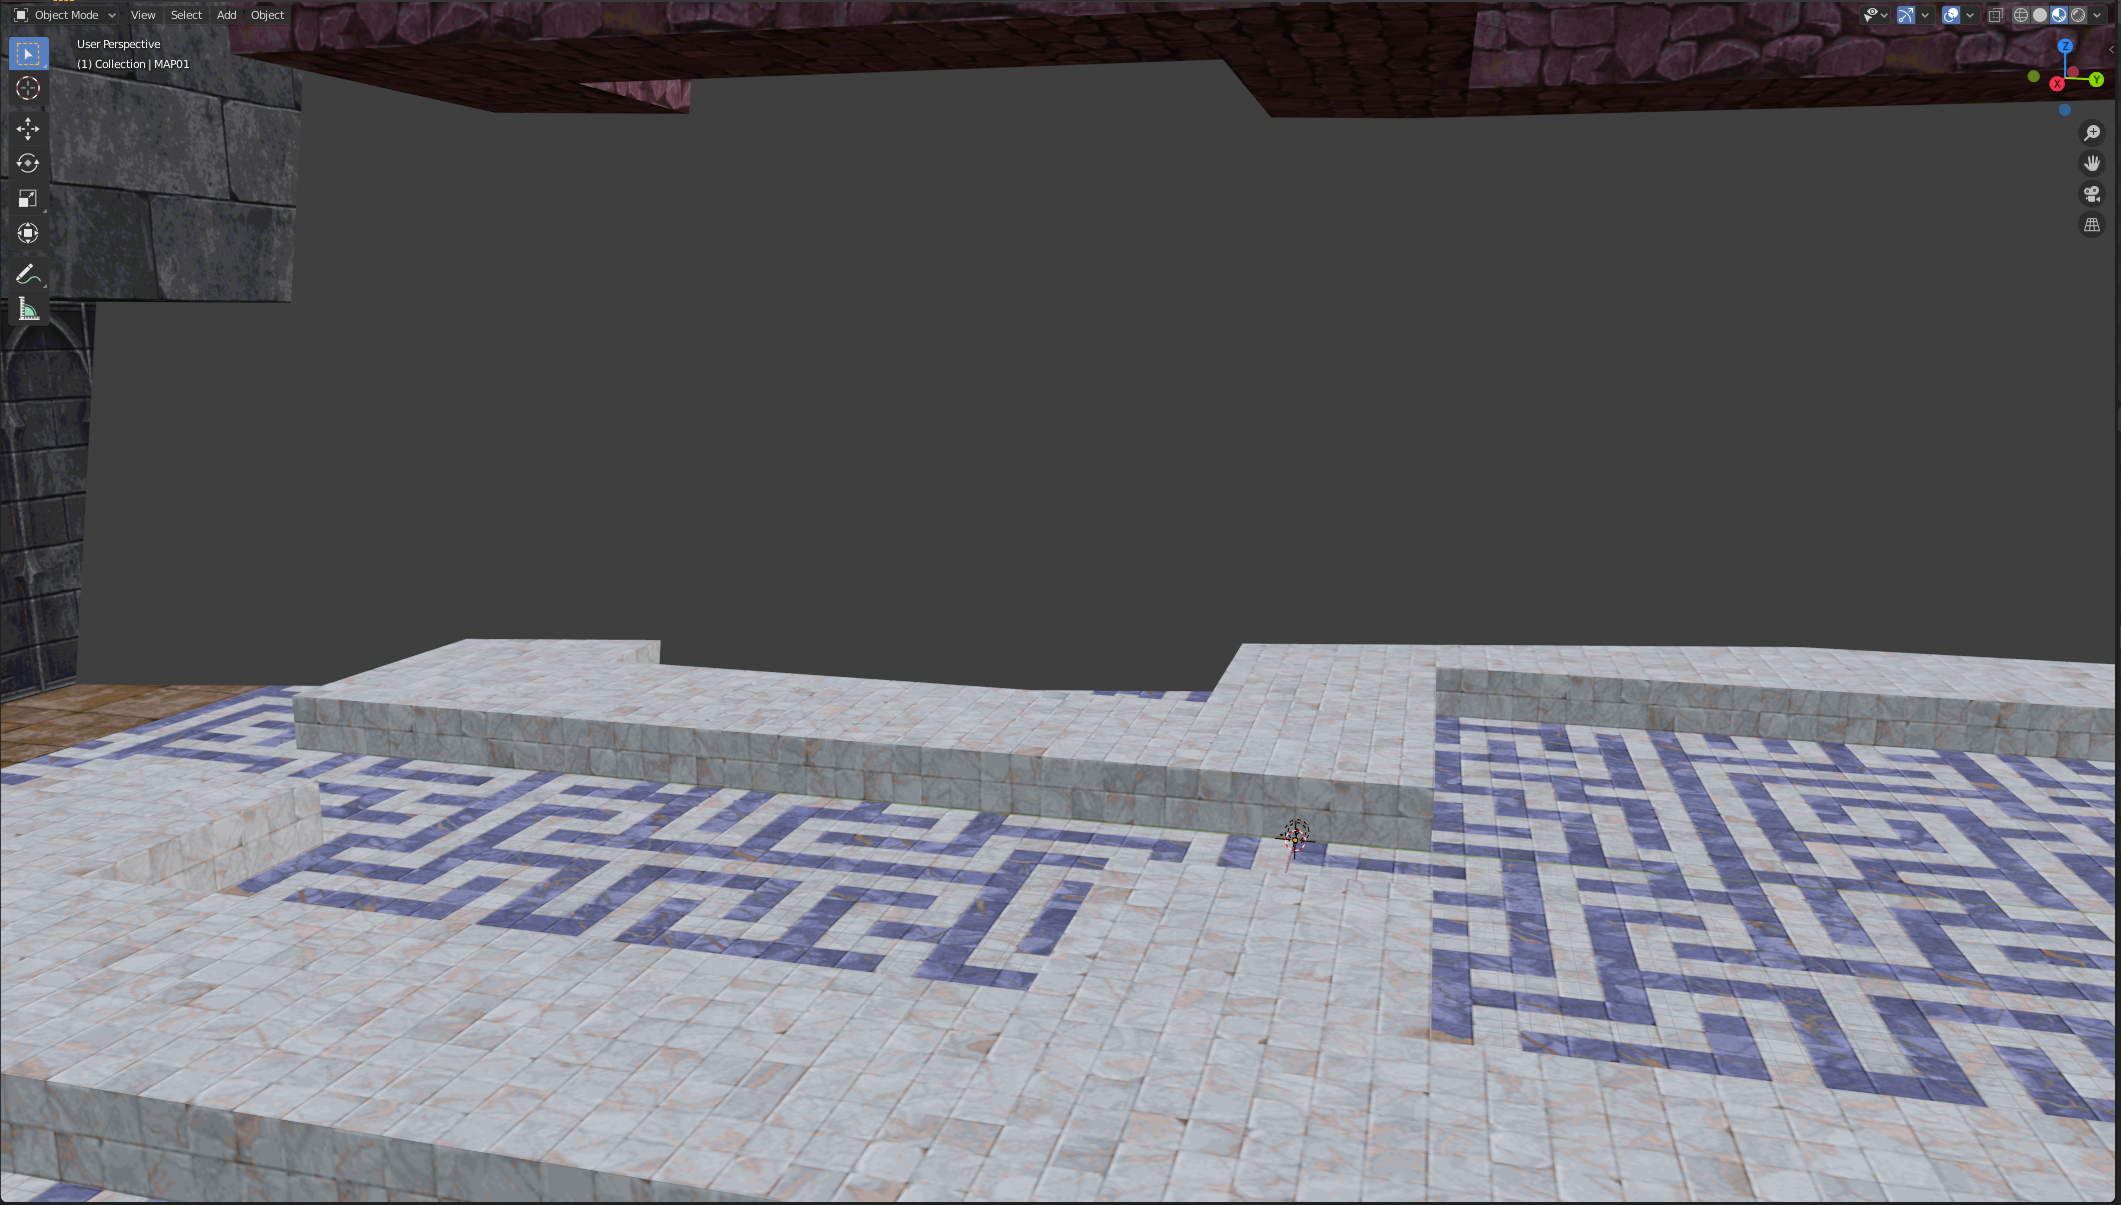
\includegraphics[height=.25\linewidth]{figures/test_map_blender.png}
	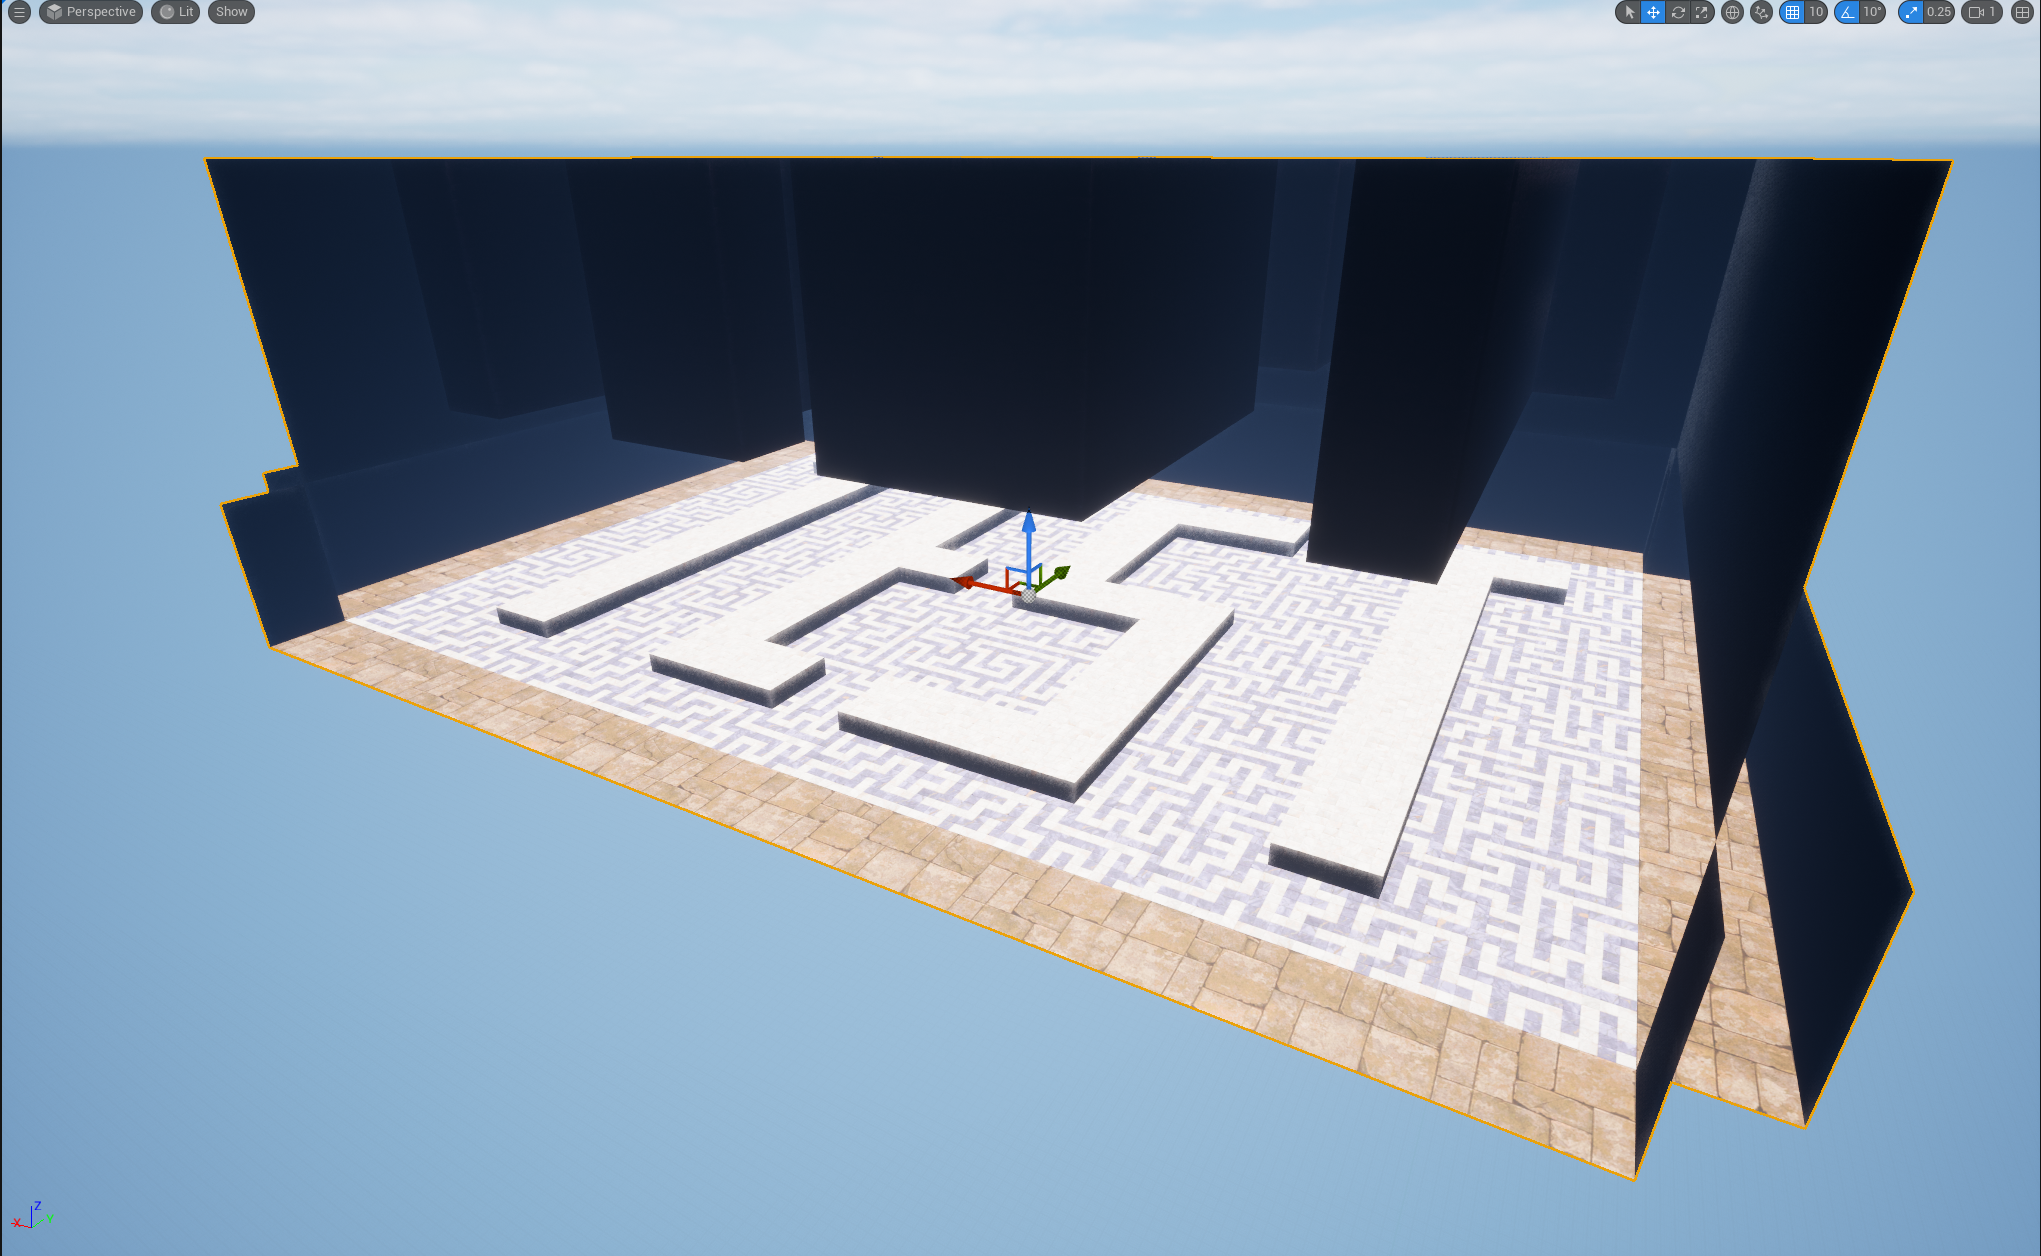
\includegraphics[height=.25\linewidth]{figures/test_map_unreal.png}
}

\frameT{Demo}{
Demo of the player in the game environment.
	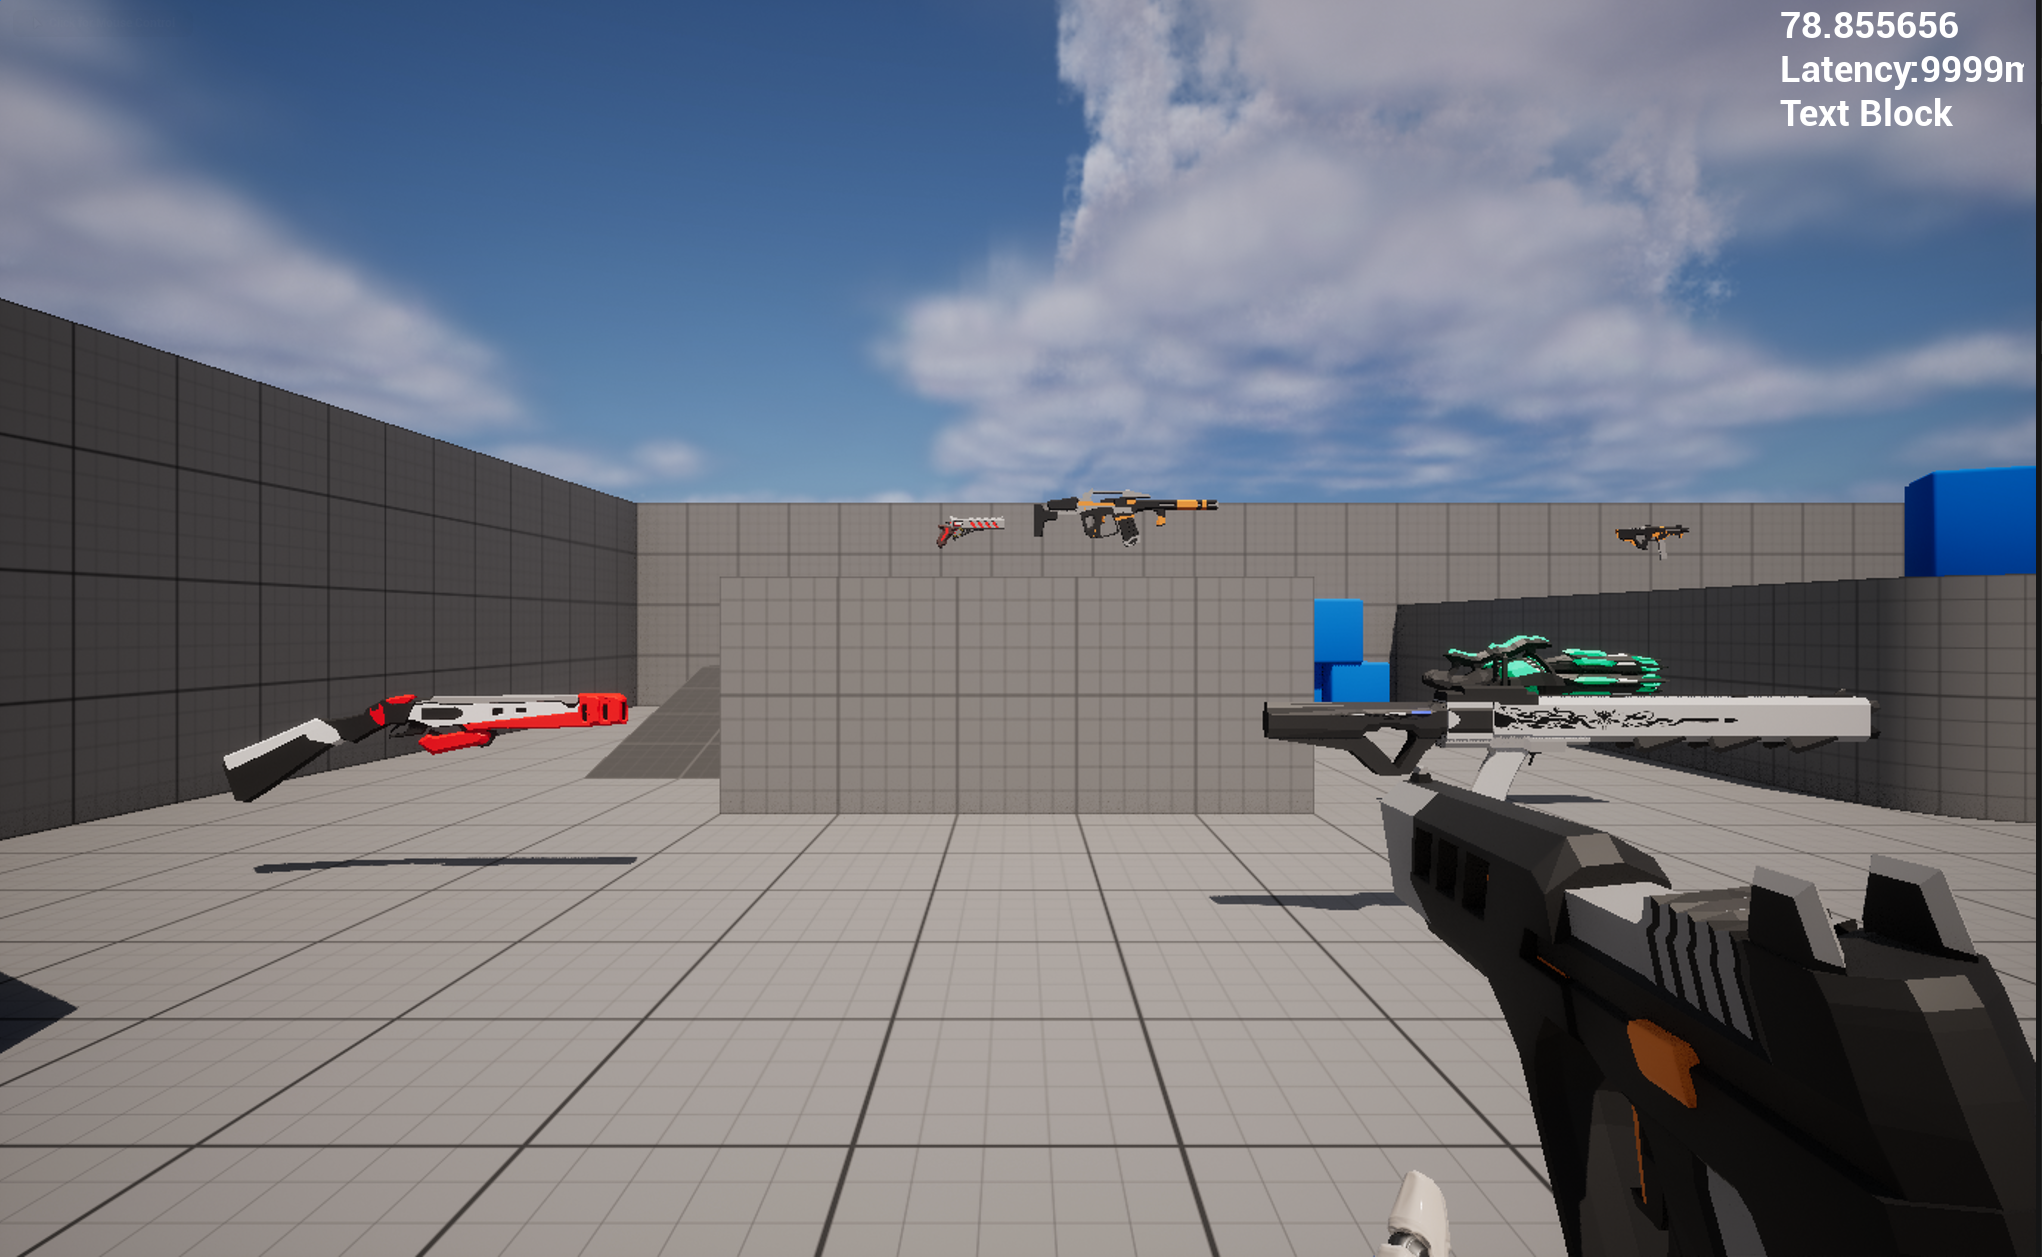
\includegraphics[height=.25\linewidth]{figures/TestDemoGame.png}
}


%\Test Online Video!!!!
%\frameT{Demo}{
%\  Demo of the player in the game environment.
  
%\  \bigskip
  
%\  \href{https://www.youtube.com/watch?v=B03EBcuClKs&ab_channel=JaxxonWoods}{Incase of Emergencies}
%\}








%\begin{frame}[fragile]
%\frametitle{Family Tree Knowledge Base}
%Facts:
%\begin{verbatim}
%Verbatim is a great way of enumerating code/algorithmic ideas.
%\end{verbatim}
%\end{frame}
%
%
%\frameT{How to include images} {
%  %% 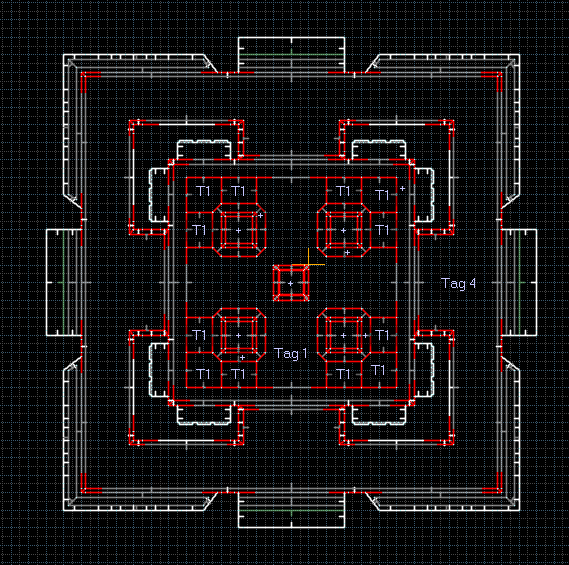
\includegraphics[width=.7\linewidth]{figures/image.pdf}
%}
%
%
%\begin{frame}[fragile]
%  \frametitle{Social Network Graph}
%  \begin{figure}[ht]
%    \begin{minipage}[b]{0.53\linewidth}
%      \centering
%      Minipages are a great way to
%    \end{minipage}
%    \hspace{0.5cm}
%    \begin{minipage}[b]{0.4\linewidth}
%      \centering
%      Line up side-by-side content.
%
%    \end{minipage}
%  \end{figure}
%  
%\end{frame}
%
%
%\frameT{Results} {
%  Describe any results of your work here.
%
%  \bigskip
%
%  Things that worked?
%
%  \bigskip
%
%  Things that didn't work?
%}
%
%\frameT{Conclusions} {
%  Some bullet points here to wrap things up.
%}

\frameT{Any Questions?} {
  
  \begin{center}
    Questions?
  \end{center}
  \begin{center}
    Comments?
  \end{center}

  \bigskip

  Contact Info:
\begin{enumerate}
    \item Victor Gasior: vicagasi@ut.utm.edu
      \bigskip
    \item Blade Johnson: davbjohn@ut.utm.edu
    \bigskip
    \item Andrew Newbill: andjnewb@ut.utm.edu
     \bigskip
    \item Lucky Woods: lucjwood@ut.utm.edu
\end{enumerate}

}

%\frameF{fragile test} {
%}

%% \frameF{Prolog Family Tree} {
%% \begin{verbatim}
%% hello
%% \end{verbatim}



%% }

%Empty Page
%\frameT{Frame 1}{
%}  


\end{document}
